\newpage
\section{DESARROLLO Y ANÁLISIS DE RESULTADOS}

A continuación se muestran los métodos de desarrollo utilizados para resolver cada uno de los problemas planteados, así como la funciones utilizadas, el método de operación a partir de diagramas de flujo y los resultados obtenidos:

\subsection{Desarrollo de la solución}

A continuación podrá consultarse una descripción de alto nivel de cada una de las funciones implementadas para conseguir los objetivos del presente laboratorio: 

\subsubsection{Función \texttt{setup()}}
Esta función se encarga de inicializar todo lo necesario para que el proyecto funcione correctamente.Configura los pines de salida para los LEDs y de entrada para los dispositivos LCD y Serial, además inicia la comunicación con el LCD y configura el modo de operación del controlador PID en modo automático.

\subsubsection{Función \texttt{simPlanta()}}
Esta función se proporcionada por el enunciado. Simula el comportamiento térmico de un bloque de aluminio con calentamiento y enfriamiento pasivo, que vendría a tomar el comportamiento de la incubadora. Dentro de la función se calcula la temperatura del bloque de aluminio en función del tiempo, considerando la transferencia de calor desde un calentador y el enfriamiento por convección al ambiente. La función recibe como parámetro la cantidad de calor \texttt{Q} suministrado al bloque de aluminio (J/s). Esta función retorna la temperatura actual \texttt{T} del bloque de aluminio (°C).

\subsubsection{Función \texttt{LED\_control()}}
Esta función controla el encendido y apagado de los LEDs en base a la temperatura externa medida en la planta. La función recibe como parámetro \texttt{out\_temp} Temperatura de salida medida (en grados Celsius).
\subsubsection{Función \texttt{LCD\_control()}}
Esta función actualiza la pantalla LCD con las temperaturas operativa, de salida y la salida del controlador PID (Señal de control). La función recibe como parámetros \texttt{op\_temp} temperatura operativa actual (en grados Celsius), \texttt{PID} salida del controlador PID, \texttt{out\_temp} temperatura de salida actual de la planta (en grados Celsius).. 



\subsubsection{Función \texttt{serial\_com()}}
Función que imprime valores en el puerto serial. Esta función agrupa los valores de la temperatura de operación, la señal de control y la señal de salida de la planta, de forma que estos puedan ser captados y utilizados en futuro procesamiento. Cuenta con tres parámetros de tipo \texttt{double}: \texttt{op\_temp}, \texttt{PID} y \texttt{out\_temp}, los cuales representan la temperatura de referencia, la señal de control y la temperatura de salida de a planta.

\subsubsection{Función \texttt{loop()}}
\texttt{loop()} es la función principal del programa, realiza las siguientes operaciones en un ciclo continuo:
\begin{itemize}
    \item Lee el valor del potenciómetro.
    \item Mapea el valor leído a un rango de 20 a 80.
    \item Actualiza el valor de referencia del controlador PID (Setpoint).
    \item Calcula la salida del controlador PID.
    \item Convierte la salida en temperatura del controlador PID a watts.
    \item Simula el comportamiento térmico de la planta y obtiene la temperatura de salida.
    \item Controla los LEDs en función de la temperatura de salida.
    \item Actualiza la pantalla LCD si el pin de control está en estado alto.
    \item Inicia o detiene la comunicación serial si el pin de control está en estado alto.
\end{itemize}


\subsubsection{Diagrama de Flujo}
A continuación se muestra un diagrama de flujo del código en C utilizado para este laboratorio:

\begin{figure}[H]
    \centering
        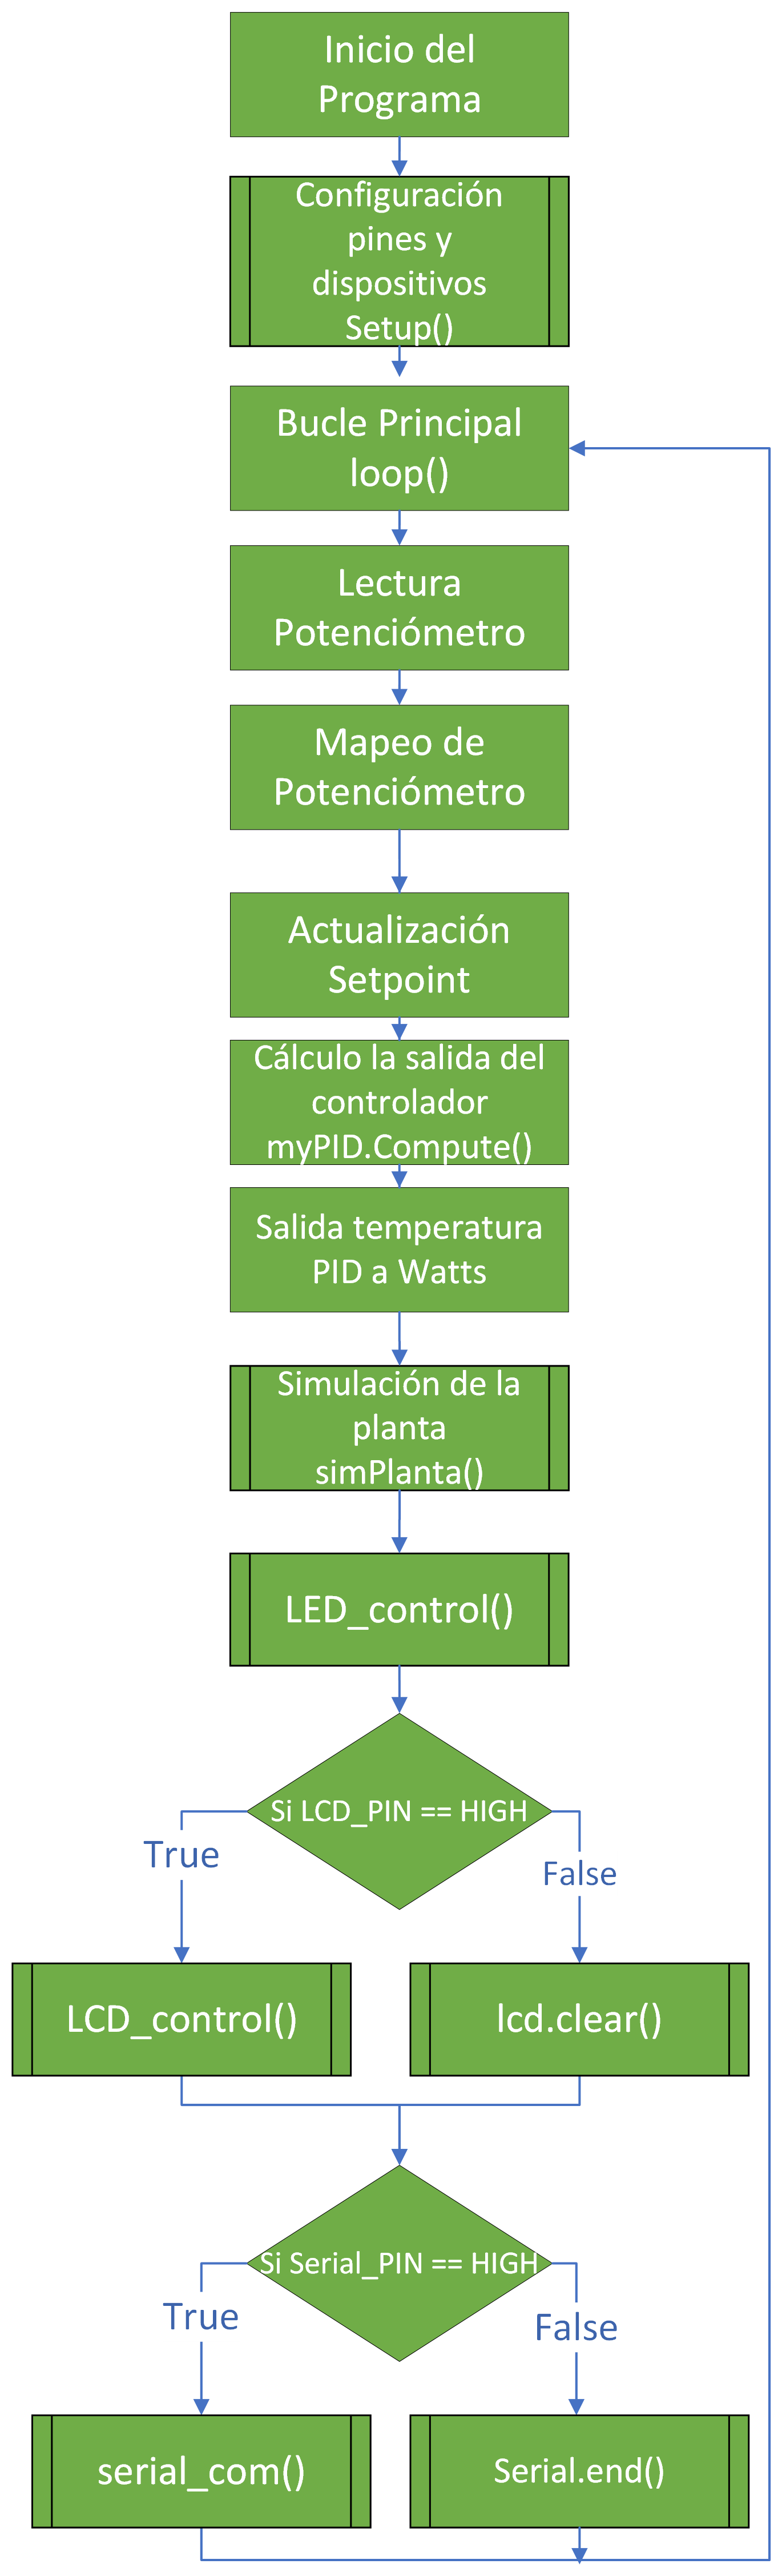
\includegraphics[scale = 0.58]{./Figuras/Desarrollo_Analisis/DF.png}
        \caption{Diagrama de flujo que describe el funcionamiento del sistema.}
    \end{figure}
\newpage


\subsubsection{\textit{Script} de Python \texttt{datasaver.py}}
Este script de Python se encarga de leer datos desde un puerto serial, el cual está conectado al Arduino UNO utilizado para realizar el proyecto, y almacenar esos datos en un archivo CSV para su posterior análisis. Primero, establece la comunicación con el puerto serial especificado y abre un archivo CSV en modo escritura. Luego, registra el tiempo inicial y entra en un bucle infinito donde lee continuamente datos del puerto serial. Cada dato es procesado para eliminar información innecesaria y se agrega el tiempo transcurrido como el primer campo. Estos datos procesados se imprimen en la terminal para verificación y se escriben en el archivo CSV. El \textit{script} opera de manera continua, asegurando una recopilación constante de datos.

\subsubsection{\textit{Script} de Python \texttt{graph.py}}
Este script de Python utiliza la biblioteca \texttt{csv} para cargar datos desde un archivo CSV y también \texttt{matplotlib.pyplot} para visualizar esos datos en forma de gráficos. Después de cargar los datos del archivo CSV en listas separadas para cada columna, utiliza \texttt{matplotlib} para graficar cada señal respecto al tiempo (primera columna). Finalmente, el \textit{script} muestra el gráfico generado. 

\subsubsection{\textit{Script} de Bash \texttt{virt\_port.sh}}
Este \textit{script} utiliza el comando \texttt{socat} para crear un puerto virtual (PTY) que enlaza dos dispositivos virtuales, \texttt{/tmp/ttyS0} y \texttt{/tmp/ttyS1}. Estos puertos virtuales se configuran para comunicarse en modo ``raw'', lo que significa que los datos se transmitirán sin procesamiento adicional. Además, se deshabilita la retroalimentación de eco (\texttt{echo=0}), lo que evita que los caracteres enviados se muestren nuevamente en el terminal. Lo anterior permite la extracción desde el Arduino. 

\subsubsection{Construcción del circuito utilizado}
Para iniciar con la construcción de este circuito, es necesario tomar en cuenta los métodos de protección descritos en las secciones \ref{sec:cir0} y \ref{sec:cir1}. Una vez que ambos fueron unidos y construidos, se conectó la salida de este circuito al pin A5 (se utiliza como pin digital), de forma que este funcionara como un interruptor para habilitar y deshabilitar la comunicación serial. Otra instancia del circuito mencionado fue conectada al pin A4 (se utiliza como pin digital) y en este caso, se utiliza para apagar y encender la pantalla LCD utilizada para mostrar las temperaturas y datos de control. El método de cálculo de las resistencias de cada LED puede observarse en la sección \ref{sec:cir2}. Por otro lado, en el caso de los LEDs utilizados para notificar del estado de la señal de salida, se utilizaron los pines D0-D2, los cuales son pines digitales y son óptimos para esta aplicación. Asimismo, en el pin A0 (utilizado como un ADC), se conectó un potenciómetro utilizado para definir la temperatura de referencia, el valor es indiferente, ya que internamente se trabaja con un mateo analógico. Finalmente, la disposición de pines para la LCD utilizada en el laboratorio también puede consultarse en la sección \ref{sec:cir2}. El circuito resultante tras implementar todas as consideraciones anteriores puede consultarse en la Figura \ref{fig:final}:

\begin{figure}[H]
\centering
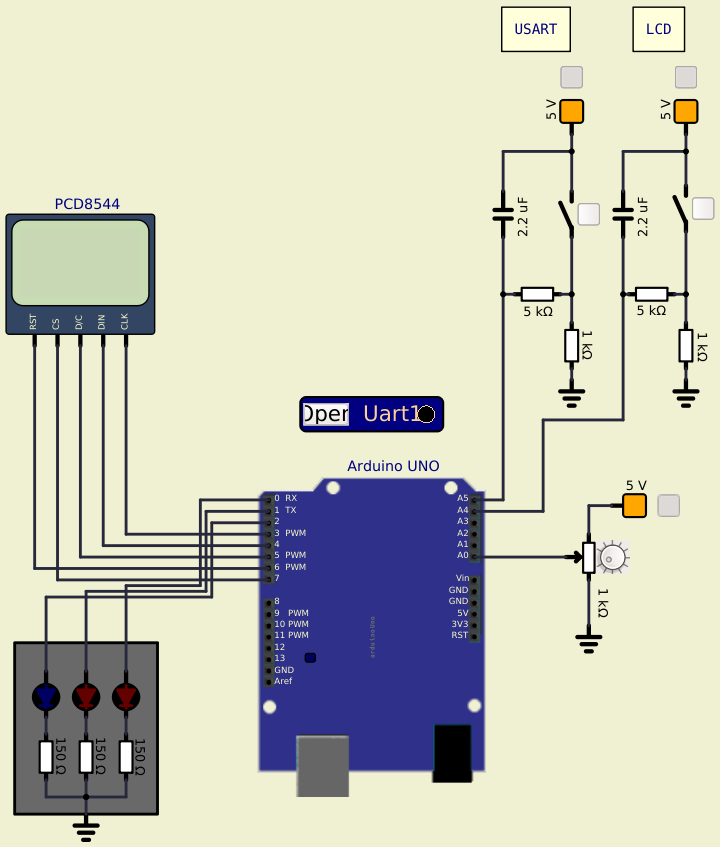
\includegraphics[width=115mm]{./Figuras/Desarrollo_Analisis/final}
\caption{Circuito final tras los cálculos de magnitudes y la implementación de las consideraciones necesarias.} 
\label{fig:final}
\end{figure}

\subsection{Análisis de los resultados}
 A continuación se mostrarán los resultados para cada una de las funcionalidades solicitadas por el enunciado: 

\subsubsection{Temperatura bajo el rango adecuado}
En la Figura \ref{fig:BR} puede observarse el comportamiento de los LEDs en función de la temperatura de salida de la planta cuando esta está por debajo del rango óptimo (30°C $\leq T \leq$ 42°C):

\begin{figure}[H]
\centering
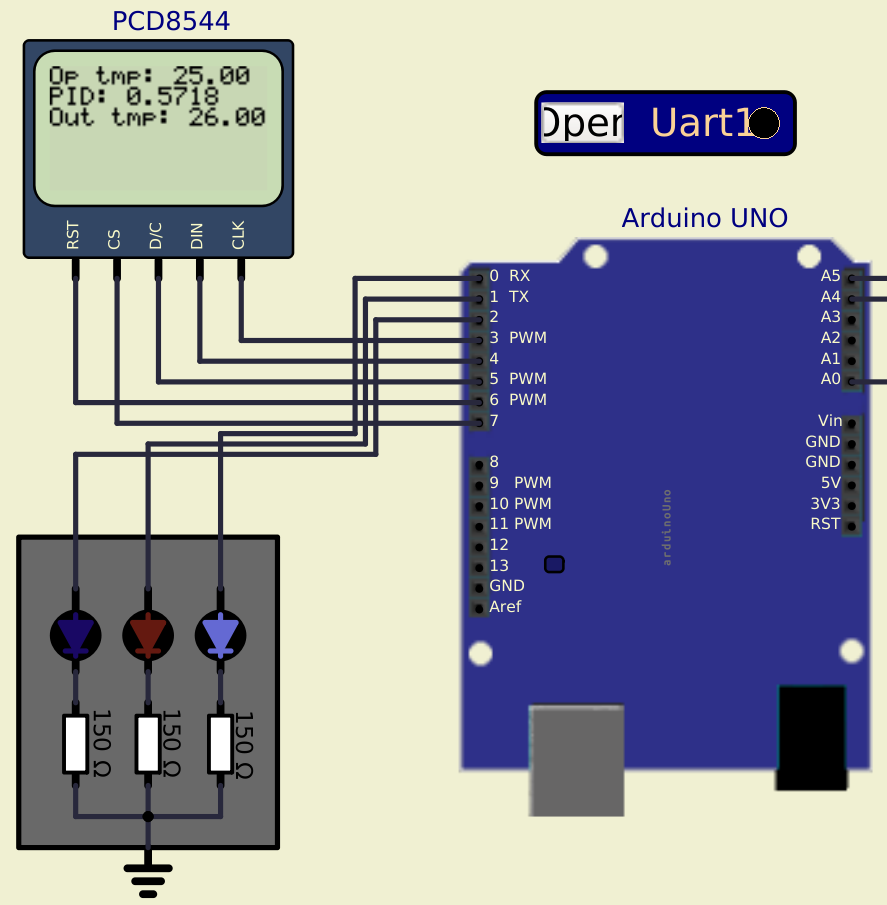
\includegraphics[width=100mm]{./Figuras/Desarrollo_Analisis/BR}
\caption{Funcionamiento del sistema cuando la temperatura de salida de la planta es inferior al rango óptimo de temperatura.} 
\label{fig:BR}
\end{figure}

Como puede verse en la Figura \ref{fig:BR}, el LED azul efectivamente se enciende cuando la temperatura de salida de la planta se encuentra en por debajo del rango óptimo.

\subsubsection{Temperatura dentro del rango adecuado}
En la Figura \ref{fig:DR} puede observarse el comportamiento de los LEDs en función de la temperatura de salida de la planta cuando esta está dentro del rango óptimo (30°C $\leq T \leq$ 42°C):

\begin{figure}[H]
\centering
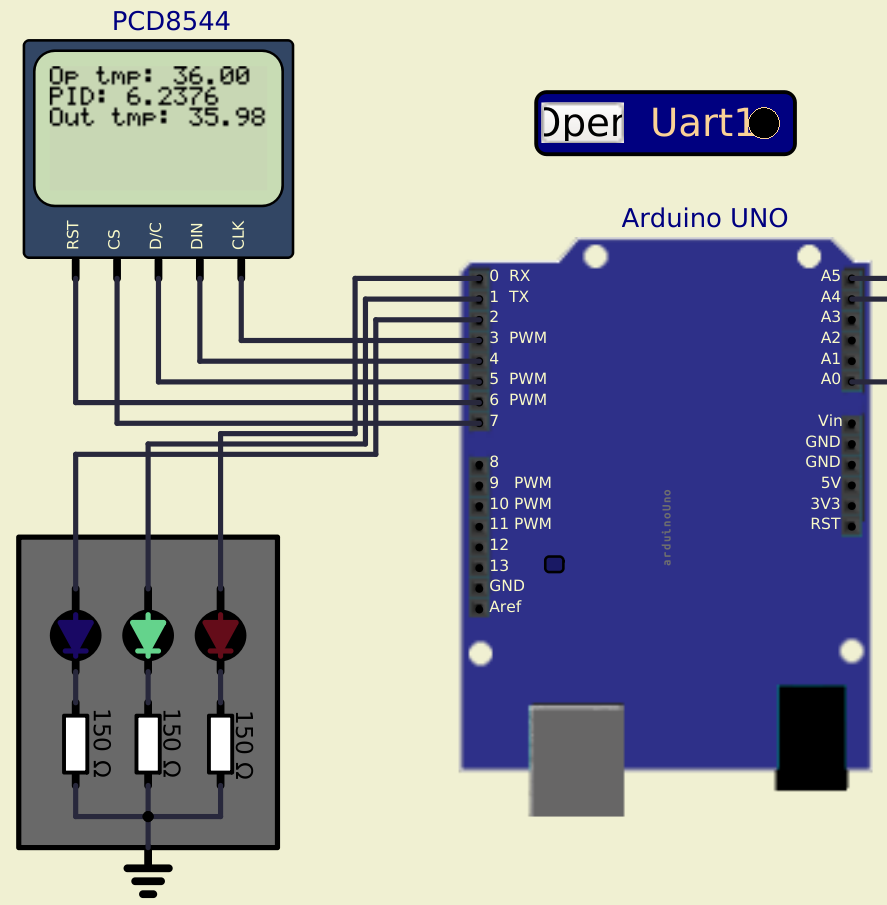
\includegraphics[width=100mm]{./Figuras/Desarrollo_Analisis/DR}
\caption{Funcionamiento del sistema cuando la temperatura de salida de la planta se encuentra dentro al rango óptimo de temperatura.} 
\label{fig:DR}
\end{figure}

Como puede verse en la Figura \ref{fig:DR}, el LED verde efectivamente se enciende cuando la temperatura de salida de la planta se encuentra dentro del rango óptimo.

\subsubsection{Temperatura sobre el rango adecuado}
En la Figura \ref{fig:DR} puede observarse el comportamiento de los LEDs en función de la temperatura de salida de la planta cuando esta está por encima del rango óptimo (30°C $\leq T \leq$ 42°C):

\begin{figure}[H]
\centering
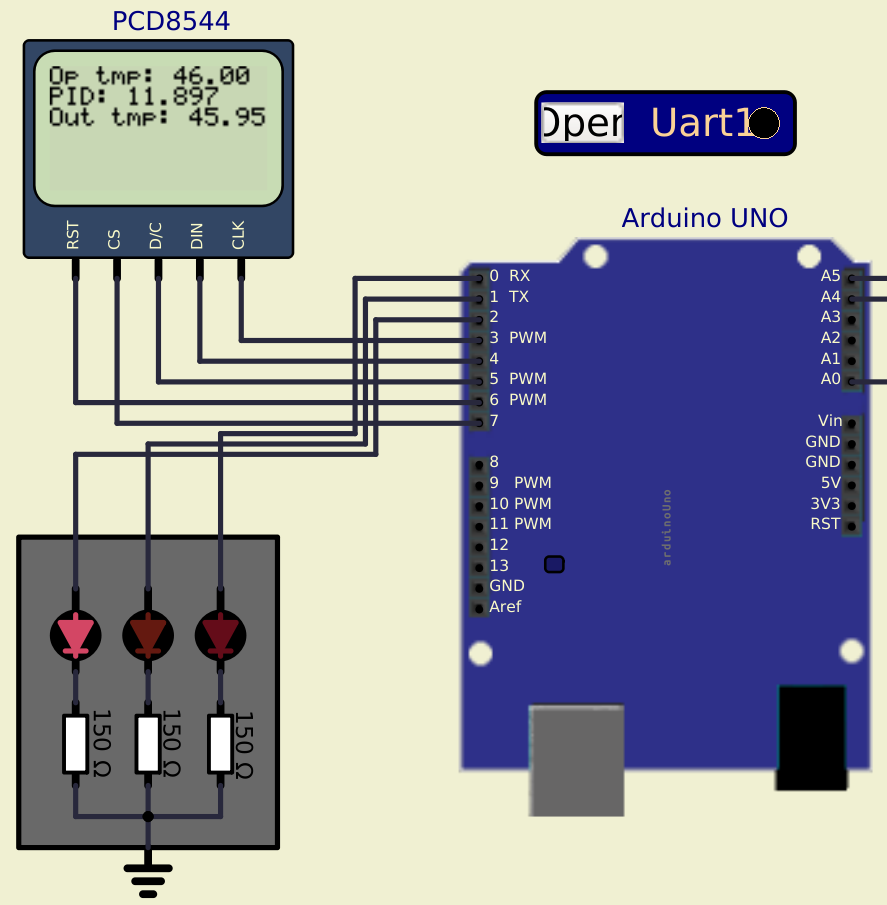
\includegraphics[width=100mm]{./Figuras/Desarrollo_Analisis/SR}
\caption{Funcionamiento del sistema cuando la temperatura de salida de la planta es superior al rango óptimo de temperatura.} 
\label{fig:SR}
\end{figure}

Como puede verse en la Figura \ref{fig:SR}, el LED rojo efectivamente se enciende cuando la temperatura de salida de la planta se encuentra en por encima del rango óptimo.

\subsubsection{Desactivación de la pantalla}
En la Figura \ref{fig:DP} puede observarse el comportamiento del sistema cuando el \textit{switch} que activa la pantalla no fue activado: 

\begin{figure}[H]
\centering
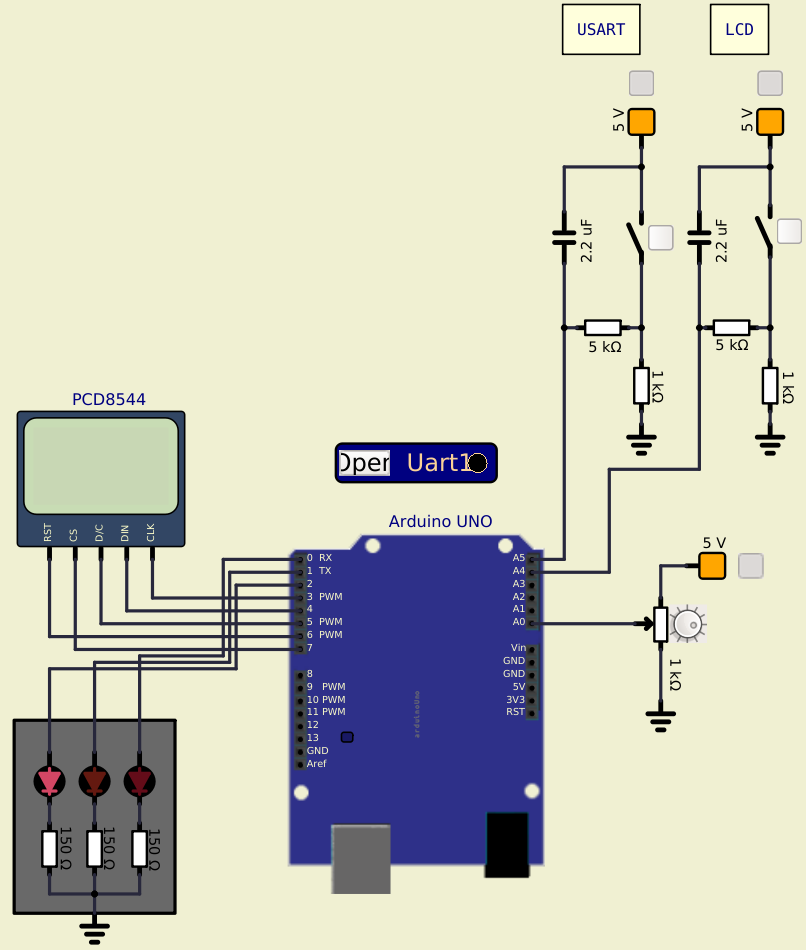
\includegraphics[width=115mm]{./Figuras/Desarrollo_Analisis/DP}
\caption{Funcionamiento de la pantalla LCD cuando el \textit{switch} encargado de gestionarla no fue activado.} 
\label{fig:DP}
\end{figure}

Como puede verse en la Figura \ref{fig:DP}, si el \textit{switch} encargado de gestionar el funcionamiento de la pantalla no ha sido activado, esta no proyecta ninguna información y se mantiene apagada, a pesar de que puede verse que el circuito sigue en funcionamiento, ya que el LED rojo está encendido, indicando que se está trabajando en una temperatura superior al rango óptimo.

\subsubsection{Desactivación de la comunicación serial}
A continuación puede verse el estado de la comunicación serial cuando el \textit{switch} que activa la comunicación serial no fue activado (Figura \ref{fig:DS1}) y el caso contrario (Figura \ref{fig:DS2}): 

\begin{figure}[H]
\centering
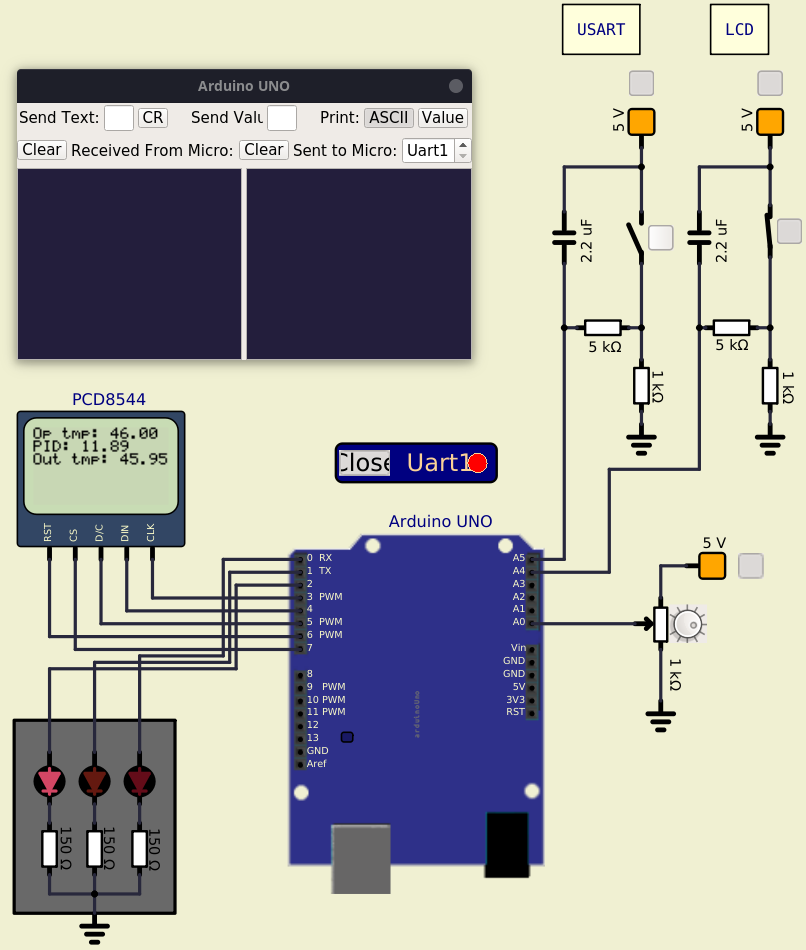
\includegraphics[width=115mm]{./Figuras/Desarrollo_Analisis/DS1}
\caption{Funcionamiento de la salida de datos por el puerto serial cuando el \textit{switch} encargado de gestionarlo no fue activado.} 
\label{fig:DS1}
\end{figure}

\begin{figure}[H]
\centering
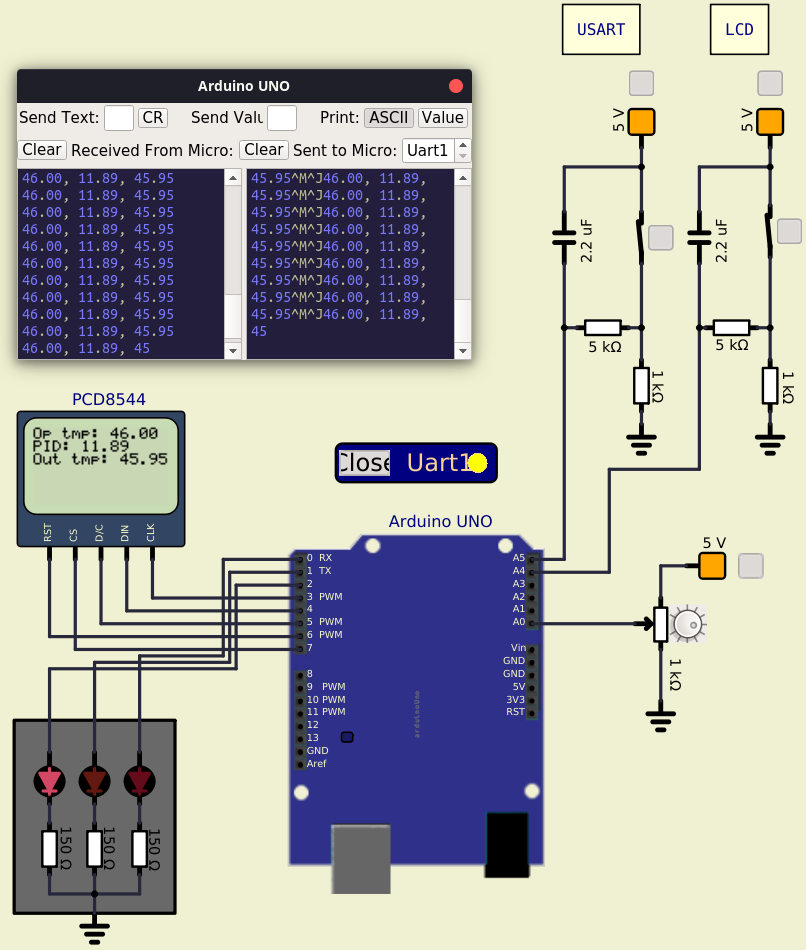
\includegraphics[width=115mm]{./Figuras/Desarrollo_Analisis/DS2}
\caption{Funcionamiento de la salida de datos por el puerto serial cuando el \textit{switch} encargado de gestionarlo fue activado.} 
\label{fig:DS2}
\end{figure}

Como puede verse en las Figuras \ref{fig:DS1} y \ref{fig:DS2}, si el \textit{switch} encargado de gestionar el funcionamiento de la comunicación serial ha sido activado, los datos recopilados por el Arduino son transportados a la computadora a través del puerto virtual y en caso contrario, esto no ocurre. 

\subsubsection{Aumento de temperatura}
A continuación pueden observarse el punto de inicio y final (Figuras \ref{fig:AT1} y \ref{fig:AT2}) y el comportamiento de las señales de temperatura de referencia, señal de control y temperatura de salida antes una disminución en la temperatura (Figura \ref{fig:AT}):

\begin{figure}[H]
\centering
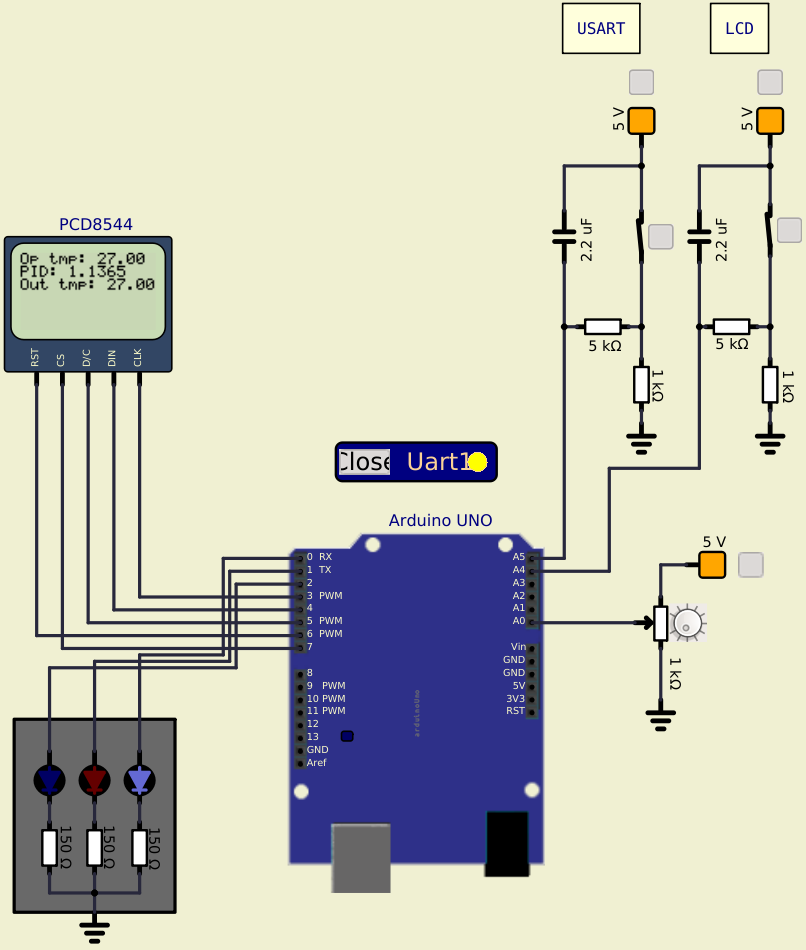
\includegraphics[width=115mm]{./Figuras/Desarrollo_Analisis/AT1}
\caption{Temperatura de inicio antes del aumento.} 
\label{fig:AT1}
\end{figure}

\begin{figure}[H]
\centering
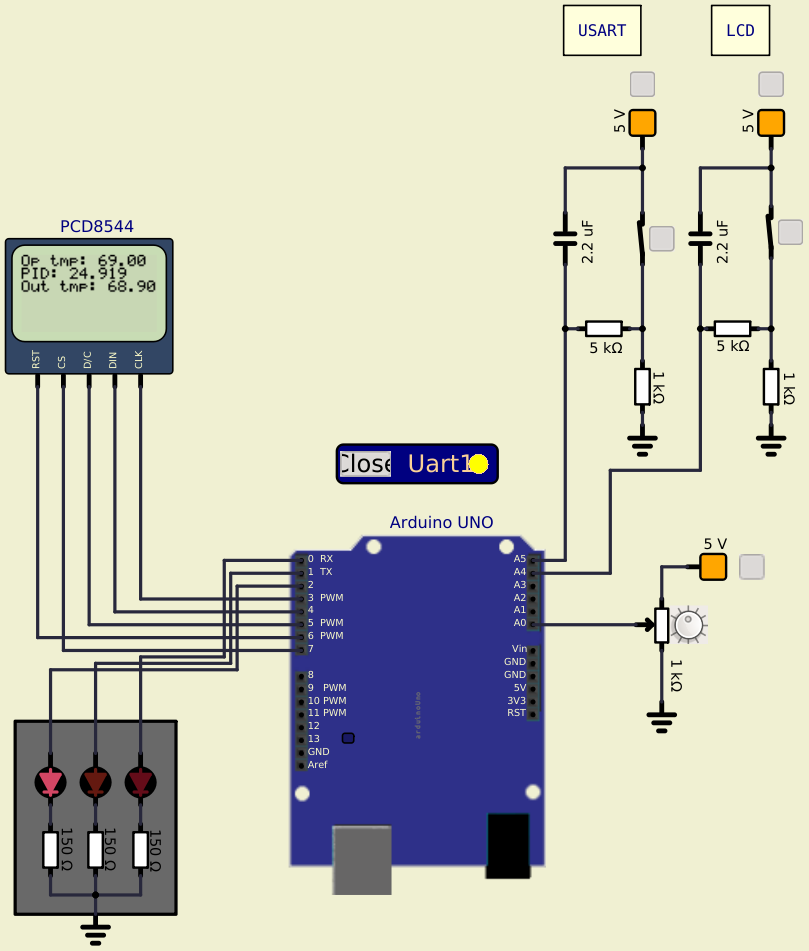
\includegraphics[width=115mm]{./Figuras/Desarrollo_Analisis/AT2}
\caption{Temperatura de final tras el aumento.} 
\label{fig:AT2}
\end{figure}

\begin{figure}[H]
\centering
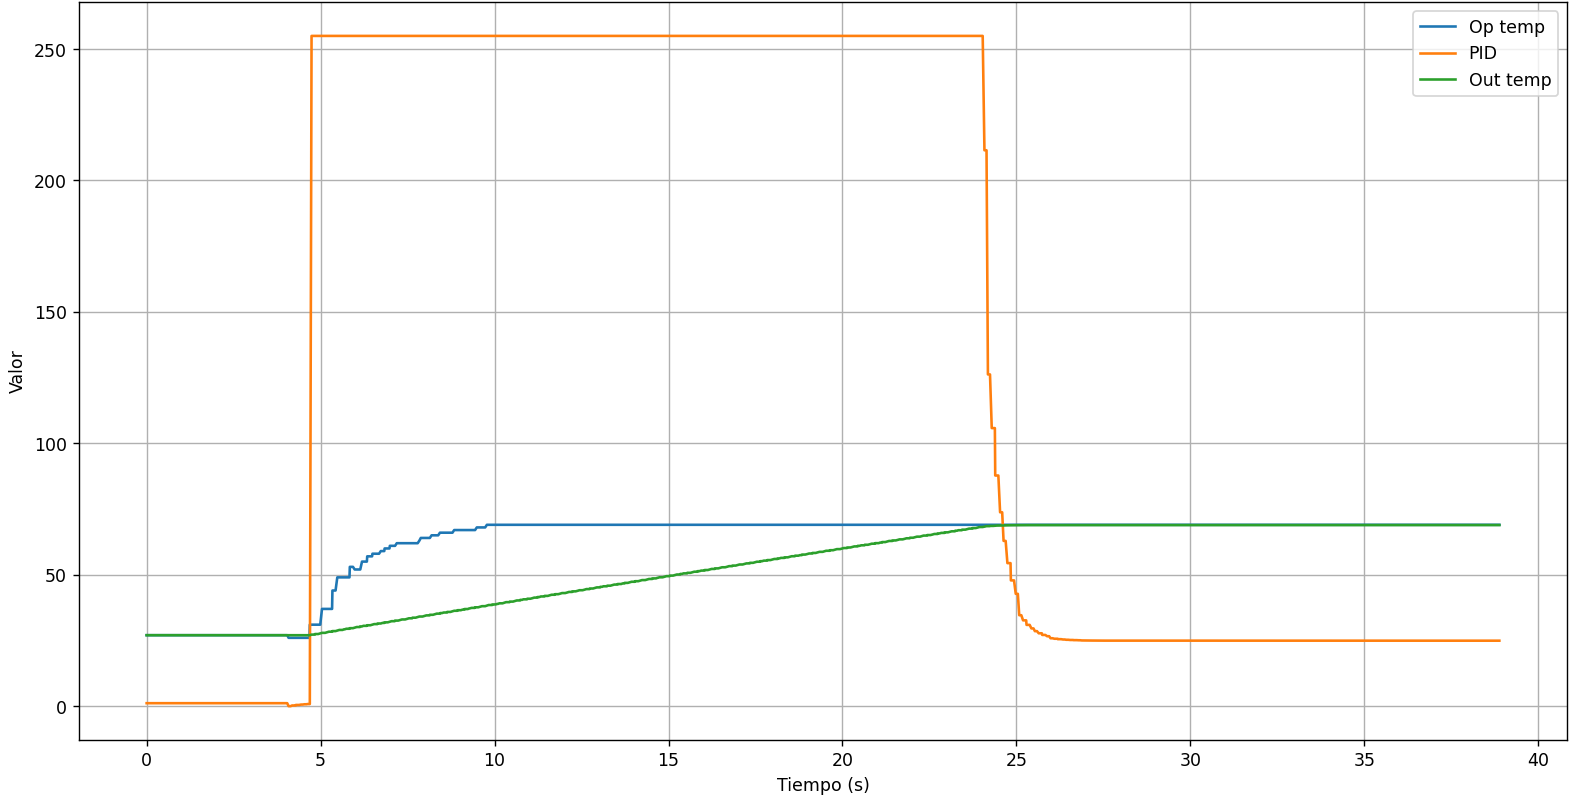
\includegraphics[width=115mm]{./Figuras/Desarrollo_Analisis/AT}
\caption{Gráfica de aumento de temperatura para cada una de las señales de interés.} 
\label{fig:AT}
\end{figure}

Como puede verse en la gráfica de la Figura \ref{fig:AT}, la temperatura de salida sigue rápidamente a la temperatura de referencia, lo cual es un comportamiento esperado (la temperatura debería subir relativamente rápido). Asimismo, se puede ver como la señal de control sube considerablemente para compensar el cambio en la referencia y baja en el momento en el que la señal de salida alcanza el \textit{setpoint}. En la Figura \ref{fig:AT2} puede verse como la temperatura de salida se aproxima casi de manera absoluta a la referencia. 

\subsubsection{Disminución de temperatura}
A continuación pueden observarse el punto de inicio y final (Figuras \ref{fig:DT1} y \ref{fig:DT2}) y el comportamiento de las señales de temperatura de referencia, señal de control y temperatura de salida antes una disminución en la temperatura (Figura \ref{fig:DT}): 

\begin{figure}[H]
\centering
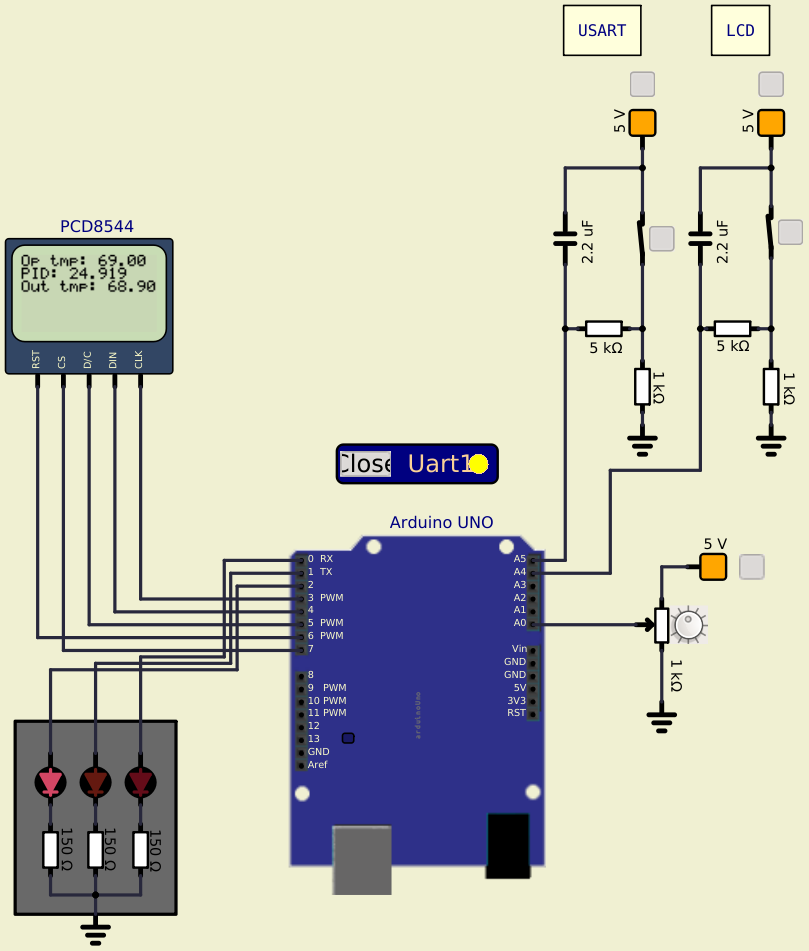
\includegraphics[width=115mm]{./Figuras/Desarrollo_Analisis/AT2}
\caption{Temperatura de inicio antes de la disminución.} 
\label{fig:DT1}
\end{figure}

\begin{figure}[H]
\centering
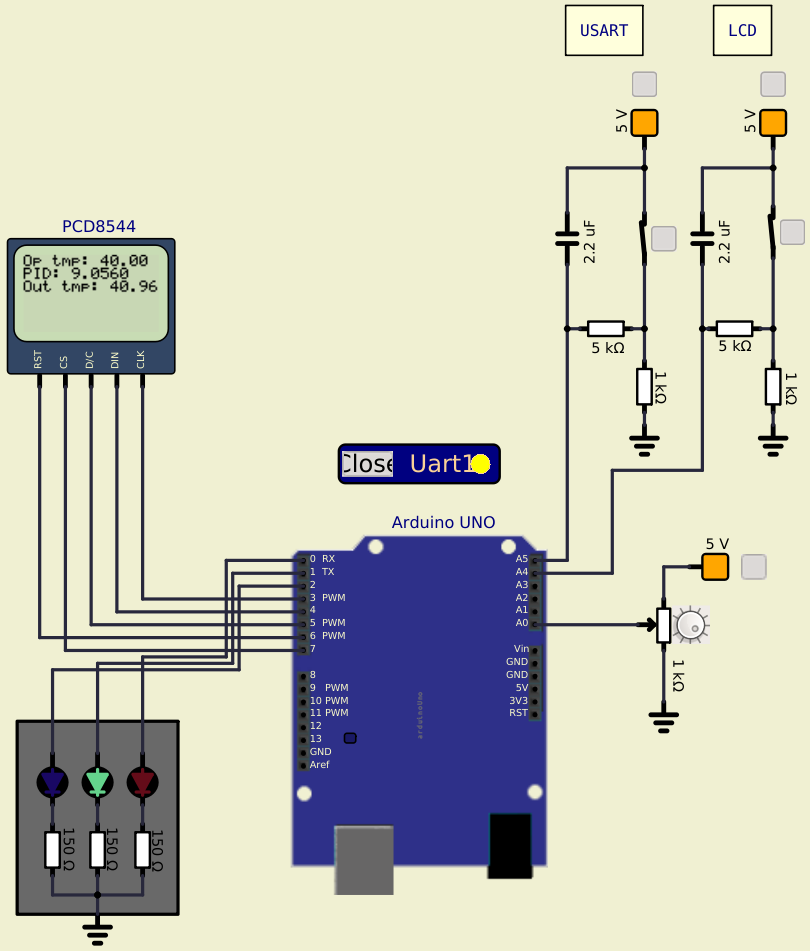
\includegraphics[width=115mm]{./Figuras/Desarrollo_Analisis/DT2}
\caption{Temperatura de final tras la disminución.} 
\label{fig:DT2}
\end{figure}

\begin{figure}[H]
\centering
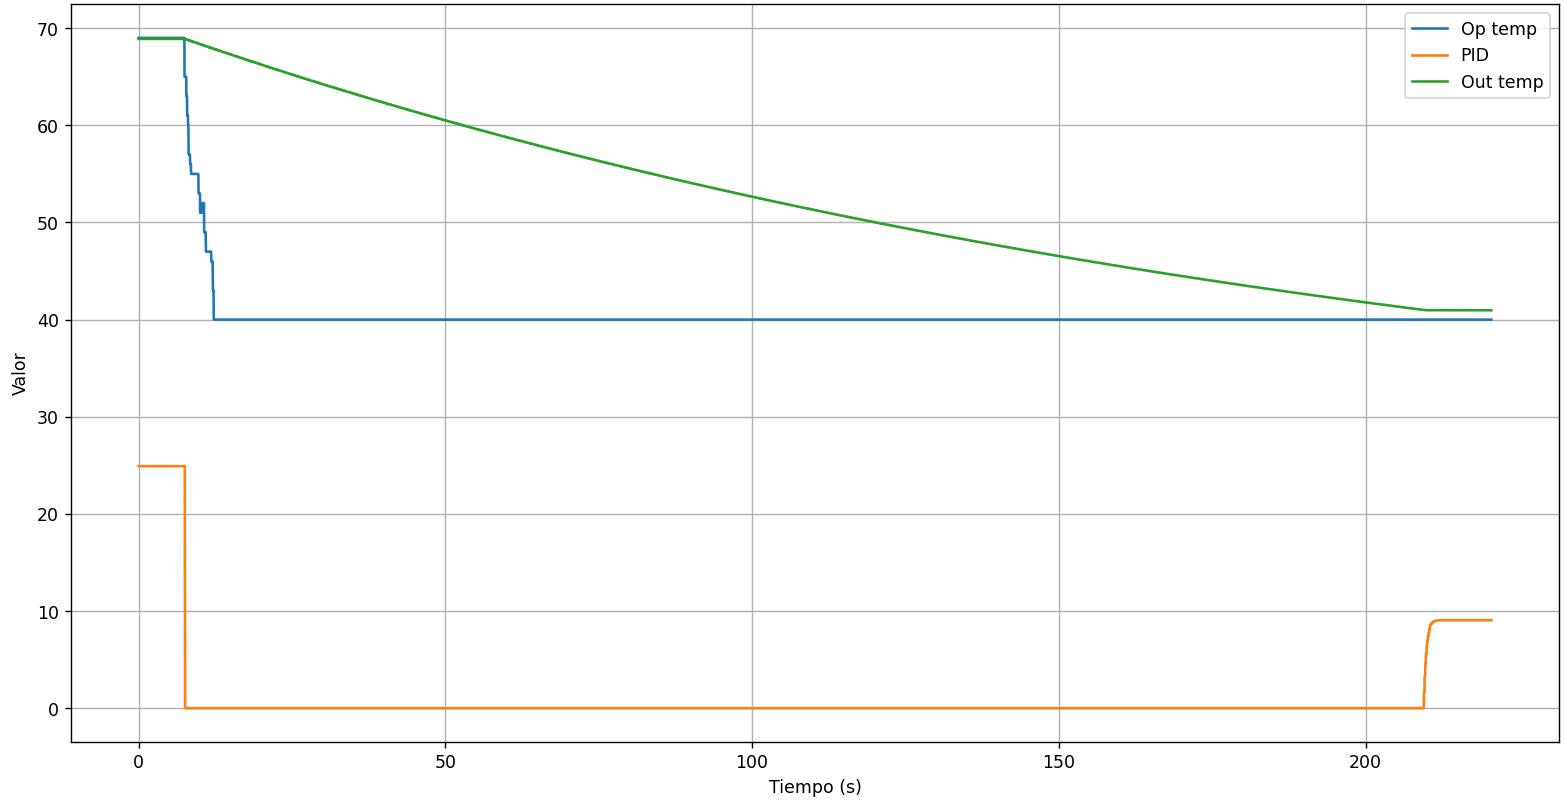
\includegraphics[width=115mm]{./Figuras/Desarrollo_Analisis/DT}
\caption{Gráfica de disminución de temperatura para cada una de las señales de interés.} 
\label{fig:DT}
\end{figure}

Como puede verse en la gráfica de la Figura \ref{fig:AT}, la temperatura de salida sigue lentamente a la temperatura de referencia, lo cual es un comportamiento esperado (la temperatura debería bajar relativamente lento). Asimismo, se puede ver como la señal de control baja para compensar el cambio en la referencia y sube en el momento en el que la señal de salida alcanza el \textit{setpoint}. En la Figura \ref{fig:DT2} puede verse como la temperatura de salida se aproxima casi de manera absoluta a la referencia. 
